\documentclass[c,unicode,russian]{beamer}
\usepackage{hyperref}
\usepackage{alltt}
\usepackage{verbatim}
\usepackage{fancyvrb}

\usepackage{fontspec}
\setsansfont{Ubuntu}
\setmonofont{Ubuntu Mono}
\usepackage{polyglossia}
\setdefaultlanguage{russian}

\useinnertheme{metropolis}
\useoutertheme{metropolis}
\usecolortheme{metropolis}

\usepackage{listings}   % C++ code
\usepackage{xcolor}     % C++ code
\lstset{%
    keywordstyle=\color{blue},
    commentstyle=\color[rgb]{0.13,0.54,0.13},
    backgroundcolor=\color{yellow!10},
    basicstyle=\small\tt,
    stringstyle=\color{red}\ttfamily,
    belowcaptionskip=-1pt,
    xleftmargin=-15pt,
    framexleftmargin=-15pt,
    framexrightmargin=5pt,
    framextopmargin=5pt,
    framexbottommargin=5pt,
    framesep=0pt,
    rulesep=0pt
}
\lstdefinestyle{cpp}{%
    language=C++,
    morecomment=[l][\color{magenta}]{\#}
}
\lstdefinestyle{python}{%
    language=Python
}

\usepackage{caption}
\renewcommand{\lstlistingname}{Код} % Listing -> Algorithm
\DeclareCaptionFont{white}{\color{white}}
\DeclareCaptionFormat{listing}{\colorbox{gray}{\parbox{\textwidth}{#1#2#3}}}
\captionsetup[lstlisting]{format=listing,labelfont=white,textfont=white}

% logo of my university
\titlegraphic{\hspace{-1cm}
\includegraphics[width=2.5in]{../../_static/logo.jpg}}

\date{}
\author{Основы Веб-программирования}
\institute{Кафедра Интеллектуальных Информационных Технологий, ИнФО, УрФУ}

\usepackage{array}      % Table

\title{Сокеты}

\begin{document}

% Slide #1
\frame{\titlepage}

% Slide #2
\begin{frame}{Ресурсы}
    \url{https://ru.wikipedia.org/wiki/Сокеты\_Беркли}\newline
    \url{http://lecturesnet.readthedocs.org/net/low-level/index.html}
\end{frame}

% Slide #3
\begin{frame}{Сокет}
    Сокет — абстрактный объект, представляющий конечную точку соединения.

    В ОС объект сокета представлен файловым дескриптором и может принимать те
    же операции что и файл (открытие - чтение/запись - закрытие).

    Дополнительно  сокеты имеют операции для связи их с адресом и подготовки к
    обмену данными.
\end{frame}

% Slide #4
\begin{frame}{Типы}
    \begin{itemize}
        \item UNIX - для взаимодействия процессов на локальной машине.
        \item INET - для взаимодействия по сети.
        \item WebSocket - протокол напоминающий механизм сокетов, предназначен
            для связи браузера с сервером (в обе стороны).
    \end{itemize}
\end{frame}

% Slide #5
\begin{frame}{INET типы}
    \begin{itemize}
        \item Stream socket - TCP.
        \item Datagram socket - UDP.
        \item Raw socket - формируем пакеты вручную.
    \end{itemize}
\end{frame}

% Slide #6
\begin{frame}[fragile]{Системный вызов socket}

    Пример INET сокета типа TCP:

    \begin{lstlisting}[style=cpp, caption=Си]
    #include <sys/types.h>
    #include <sys/socket.h>
    int sock_fd = socket(AF_INET, SOCK_STREAM, 0);
    \end{lstlisting}

    \begin{lstlisting}[style=python, caption=Python]
    import socket
    sock_obj = socket.socket(socket.AF_INET,
                             socket.SOCK_STREAM, 0)
    \end{lstlisting}
\end{frame}

% Slide #7
\begin{frame}{Основные функции}
    \begin{center}
        \begin{tabular}{| m{5em} | m{22em}|}
            \hline
            socket  & Создать новый сокет и вернуть файловый дескриптор \\
            \hline
            send    & Отправить данные по сети \\
            \hline
            receive & Получить данные из сети \\
            \hline
            close   & Закрыть соединение \\
            \hline
            bind    & Связать сокет с IP-адресом и портом \\
            \hline
            listen  & Объявить о желании принимать соединения. Слушает порт и
                        ждет когда будет установлено соединение \\
            \hline
            accept  & Принять запрос на установку соединения \\
            \hline
            connect & Установить соединение  \\
            \hline
        \end{tabular}
    \end{center}
\end{frame}

% Slide #8
\begin{frame}[fragile]{Клиент. Установка соединения}

    Со стороны клиента используется функция \textbf{connect}, которая
    инициирует установление связи на сокете:

    \begin{lstlisting}[style=cpp, caption=Си]
    #include <sys/types.h>
    #include <sys/socket.h>
    int connect(int sockfd,
                const struct sockaddr *serv_addr,
                socklen_t addrlen);
    \end{lstlisting}

    \begin{lstlisting}[style=python, caption=Python]
    server_address = ('192.168.1.100', 8080)
    sock_obj.connect(server_address)
    \end{lstlisting}
\end{frame}

% Slide #9
\begin{frame}[fragile]{Клиент. Установка соединения}

    Со стороны клиента используется функция \textbf{connect}:

    \begin{lstlisting}[style=cpp, caption=Си]
    #include <sys/types.h>
    #include <sys/socket.h>
    int connect(int sockfd,
                const struct sockaddr *serv_addr,
                socklen_t addrlen);
    \end{lstlisting}

    \begin{lstlisting}[style=python, caption=Python]
    server_address = ('192.168.1.100', 8080)
    sock_obj.connect(server_address)
    \end{lstlisting}
\end{frame}

% Slide #10
\begin{frame}{Сервер. Установка соединения}

    Сервер слушает порт и при запросе от клиента устанавливает
    соединение.

    \begin{center}
        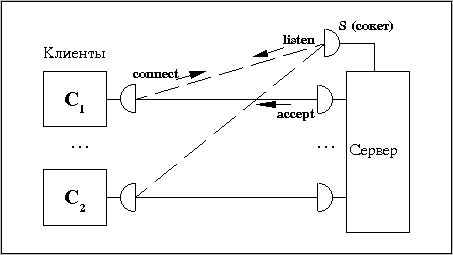
\includegraphics[width=4.2in]{media/socket-server.png}
    \end{center}
\end{frame}

% Slide #11
\begin{frame}[fragile]{Сервер. Ждем соединения.}
    Сервер слушает порт и ожидает запрос на соединение от клиента:

    \begin{lstlisting}[style=cpp, caption=Си]
    #include <sys/socket.h>
    int listen(int sockfd, int backlog);
    \end{lstlisting}

    \begin{lstlisting}[style=python, caption=Python]
    sock_obj.listen(5)  # fd = 5
    \end{lstlisting}
\end{frame}

% Slide #12
\begin{frame}[fragile]{Сервер. Подтверждаем соединение.}

    \textbf{accept} - подтверждает запрос клиента и устанавливает соединение.

    \begin{lstlisting}[style=cpp, caption=Си]
    #include <sys/types.h>
    #include <sys/socket.h>
    int accept(int sockfd, struct sockaddr *cliaddr,
               socklen_t *addrlen);
    \end{lstlisting}

    \begin{lstlisting}[style=python, caption=Python]
    conn, addr = sock_obj.accept()
    \end{lstlisting}
\end{frame}

% Slide #13
\begin{frame}[fragile]{Передача данных}

    В Python вызов методов \textbf{send}, \textbf{recv} без дополнительных
    параметров, аналогичен системным вызовам \textbf{read}, \textbf{write}.

    \begin{lstlisting}[style=cpp, caption=Си]
    #include <sys/types.h>
    #include <unistd.h>
    ssize_t read(int fd, void *buf, size_t nbytes);
    ssize_t write(int fd, const void *buf, size_t nbytes);
    \end{lstlisting}

    \begin{lstlisting}[style=python, caption=Python]
    conn.send('Hello World!')
    data = conn.recv(BUFFER_SIZE)
    \end{lstlisting}
\end{frame}

% Slide #14
\begin{frame}[fragile]{Сервер TCP на Pyhton}

    Создаем TCP сокет, который слушает порт 5005 на локальной машине.

    \begin{lstlisting}[style=python, caption=Python]
    import socket

    TCP_IP = '127.0.0.1'
    TCP_PORT = 5005
    BUFFER_SIZE = 20  # Normally 1024,
                      # but we want fast response
    s = socket.socket(socket.AF_INET, socket.SOCK_STREAM)
    s.bind((TCP_IP, TCP_PORT))
    s.listen(1)
    \end{lstlisting}
\end{frame}

% Slide #15
\begin{frame}[fragile]{Сервер TCP на Pyhton}

    После запроса клиента и установки с ним соединения, сервер в бесконечном
    цикле принимает от него данные, выводит их на экран и возвращает обратно.
    (Эхо-сервер)

    \begin{lstlisting}[style=python, caption=Python]
    conn, addr = s.accept()
    print("Connection address: {}".format(addr))
    while 1:
        data = conn.recv(BUFFER_SIZE)
        print("received data: {}".format(data))
        conn.send(data)  # echo
    conn.close()
    \end{lstlisting}
\end{frame}

% Slide #16
\begin{frame}[fragile]{Клиент TCP}

    TCP соединение всегда можно установить при помощи утилиты \textbf{Telnet}.

    \begin{lstlisting}[style=python, caption=Telnet]
    $ telnet localhost 5005
    \end{lstlisting}
\end{frame}

% Slide #17
\begin{frame}[fragile]{Клиент TCP на Python}

    Создаем сокет и отправляем запрос на установку соединения с сервером.

    \begin{lstlisting}[style=python, caption=Python]
    import socket

    TCP_IP = '127.0.0.1'
    TCP_PORT = 5005
    BUFFER_SIZE = 1024
    MESSAGE = "Hello, World!"

    s = socket.socket(socket.AF_INET, socket.SOCK_STREAM)
    s.connect((TCP_IP, TCP_PORT))
    \end{lstlisting}
\end{frame}

% Slide #18
\begin{frame}[fragile]{Клиент TCP на Python}

    Отправляем данные, получаем ответ сервера и закрываем соединение.

    \begin{lstlisting}[style=python, caption=Python]
    s.send(MESSAGE)
    data = s.recv(BUFFER_SIZE)
    s.close()

    print("received data: {}".format(data))
    \end{lstlisting}
\end{frame}

% Slide #19
\begin{frame}[fragile]{Клиент HTTP на Python}

    Устанавливаем TCP соединение с \textbf{httpbin.org} и отправляем строку
    запроса.

    \begin{lstlisting}[style=python, caption=Python]
    sock_obj = socket.socket(socket.AF_INET,
                             socket.SOCK_STREAM)

    sock_obj.connect(('httpbin.org', 80))
    sock_obj.send("GET /ip HTTP/1.0\n\n")
    \end{lstlisting}
\end{frame}

\end{document}
